\documentclass[12pt, titlepage]{article}

\usepackage{fullpage}
\usepackage[round]{natbib}
\usepackage{multirow}
\usepackage{booktabs}
\usepackage{tabularx}
\usepackage{graphicx}
\usepackage{float}
\usepackage{hyperref}
\hypersetup{
  colorlinks,
  citecolor=blue,
  filecolor=black,
  linkcolor=red,
  urlcolor=blue
}

%% Comments

\usepackage{color}

\newif\ifcomments\commentstrue %displays comments
%\newif\ifcomments\commentsfalse %so that comments do not display

\ifcomments
\newcommand{\authornote}[3]{\textcolor{#1}{[#3 ---#2]}}
\newcommand{\todo}[1]{\textcolor{red}{[TODO: #1]}}
\else
\newcommand{\authornote}[3]{}
\newcommand{\todo}[1]{}
\fi

\newcommand{\wss}[1]{\authornote{blue}{SS}{#1}} 
\newcommand{\plt}[1]{\authornote{magenta}{TPLT}{#1}} %For explanation of the template
\newcommand{\an}[1]{\authornote{cyan}{Author}{#1}}

%% Common Parts

\newcommand{\progname}{ProgName} % PUT YOUR PROGRAM NAME HERE
\newcommand{\authname}{Team \#, Team Name
\\ Student 1 name
\\ Student 2 name
\\ Student 3 name
\\ Student 4 name} % AUTHOR NAMES                  

\usepackage{hyperref}
    \hypersetup{colorlinks=true, linkcolor=blue, citecolor=blue, filecolor=blue,
                urlcolor=blue, unicode=false}
    \urlstyle{same}
                                


\newcounter{acnum}
\newcommand{\actheacnum}{AC\theacnum}
\newcommand{\acref}[1]{AC\ref{#1}}

\newcounter{ucnum}
\newcommand{\uctheucnum}{UC\theucnum}
\newcommand{\uref}[1]{UC\ref{#1}}

\newcounter{mnum}
\newcommand{\mthemnum}{M\themnum}
\newcommand{\mref}[1]{M\ref{#1}}

\begin{document}

\title{Module Guide for \progname{}}
\author{\authname}
\date{\today}

\maketitle

\pagenumbering{roman}

\section{Revision History}

\begin{tabularx}{\textwidth}{p{3cm}p{2cm}X}
  \toprule {\bf Date} & {\bf Version} & {\bf Notes} \\
  \midrule
  Date 1              & 1.0           & Notes       \\
  Date 2              & 1.1           & Notes       \\
  \bottomrule
\end{tabularx}

\newpage

\section{Reference Material}

This section records information for easy reference.

\subsection{Abbreviations and Acronyms}

\renewcommand{\arraystretch}{1.2}
\begin{tabular}{l l}
  \toprule
  \textbf{symbol} & \textbf{description}                \\
  \midrule
  AC              & Anticipated Change                  \\
  API             & Application Programming Interface   \\
  AWS             & Amazon Web Services                 \\
  DAG             & Directed Acyclic Graph              \\
  DB              & Database                            \\
  GPD             & Global Positioning System           \\
  JSON            & Javascript Object Notation          \\
  M               & Module                              \\
  MG              & Module Guide                        \\
  OS              & Operating System                    \\
  R               & Requirement                         \\
  REST            & Representational State Transfer     \\
  RPC             & Remote Procedure Call               \\
  SC              & Scientific Computing                \\
  SOAP            & Simple Object Access Protocol       \\
  SRS             & Software Requirements Specification \\
  \progname       & Syncing to a single source of truth \\
  UC              & Unlikely Change                     \\
  UI              & User Interface                      \\
  \bottomrule
\end{tabular}\\

\newpage

\tableofcontents

\listoftables

\listoffigures

\newpage

\pagenumbering{arabic}

\section{Introduction}

Decomposing a system into modules is a commonly accepted approach to developing
software.  A module is a work assignment for a programmer or programming
team~\citep{ParnasEtAl1984}.  We advocate a decomposition
based on the principle of information hiding~\citep{Parnas1972a}.  This
principle supports design for change, because the ``secrets'' that each module
hides represent likely future changes.  Design for change is valuable in SC,
where modifications are frequent, especially during initial development as the
solution space is explored.

Our design follows the rules layed out by \citet{ParnasEtAl1984}, as follows:
\begin{itemize}
  \item System details that are likely to change independently should be the
    secrets of separate modules.
  \item Each data structure is implemented in only one module.
  \item Any other program that requires information stored in a module's data
    structures must obtain it by calling access programs belonging to
    that module.
\end{itemize}

After completing the first stage of the design, the Software Requirements
Specification (SRS), the Module Guide (MG) is
developed~\citep{ParnasEtAl1984}. The MG
specifies the modular structure of the system and is intended to allow both
designers and maintainers to easily identify the parts of the software.  The
potential readers of this document are as follows:

\begin{itemize}
  \item New project members: This document can be a guide for a new
    project member
    to easily understand the overall structure and quickly find the
    relevant modules they are searching for.
  \item Maintainers: The hierarchical structure of the module guide improves the
    maintainers' understanding when they need to make changes to the
    system. It is
    important for a maintainer to update the relevant sections of the document
    after changes have been made.
  \item Designers: Once the module guide has been written, it can be used to
    check for consistency, feasibility, and flexibility. Designers
    can verify the
    system in various ways, such as consistency among modules,
    feasibility of the
    decomposition, and flexibility of the design.
\end{itemize}

The rest of the document is organized as follows. Section
\ref{SecChange} lists the anticipated and unlikely changes of the software
requirements. Section \ref{SecMH} summarizes the module decomposition that
was constructed according to the likely changes. Section \ref{SecConnection}
specifies the connections between the software requirements and the
modules. Section \ref{SecMD} gives a detailed description of the
modules. Section \ref{SecTM} includes two traceability matrices. One checks
the completeness of the design against the requirements provided in the SRS. The
other shows the relation between anticipated changes and the modules. Section
\ref{SecUse} describes the use relation between modules.

\section{Anticipated and Unlikely Changes} \label{SecChange}

This section lists possible changes to the system. According to the likeliness
of the change, the possible changes are classified into two
categories. Anticipated changes are listed in Section \ref{SecAchange}, and
unlikely changes are listed in Section \ref{SecUchange}.

\subsection{Anticipated Changes} \label{SecAchange}

Anticipated changes are the source of the information that is to be hidden
inside the modules. Ideally, changing one of the anticipated changes will only
require changing the one module that hides the associated decision. The approach
adapted here is called design for
change.

\begin{description}
  \item[\refstepcounter{acnum} \actheacnum \label{acGps}:] Updates to the
    GPS authentication mechanism.
  \item[\refstepcounter{acnum} \actheacnum
    \label{acLocationThreshod}:] Changes in
    the geofencing radius or conditions for location-based authentication.
  \item[\refstepcounter{acnum} \actheacnum \label{acAuthenticationMethods}:]
    Changes to user authentication methods such as the addition of one time
    passwords.
  \item[\refstepcounter{acnum} \actheacnum \label{acDocuments}:] The different
    types of supported document formats to be stored in the system.
  \item[\refstepcounter{acnum} \actheacnum \label{acIntegration}:] Incorporating
    APIs from other city management systems (e.g. Infor EAM)
  \item[\refstepcounter{acnum} \actheacnum \label{acDataLogs}:] Analytic
    information requested by administrators, such as located-based
    usage patterns.
\end{description}

\subsection{Unlikely Changes} \label{SecUchange}

The module design should be as general as possible. However, a general system is
more complex. Sometimes this complexity is not necessary. Fixing some design
decisions at the system architecture stage can simplify the software design. If
these decision should later need to be changed, then many parts of the design
will potentially need to be modified. Hence, it is not intended that these
decisions will be changed.

\begin{description}
  \item[\refstepcounter{ucnum} \uctheucnum \label{ucLocation}:]
    Removing location
    authentication features completely.
  \item[\refstepcounter{ucnum} \uctheucnum \label{ucAWS}:] AWS as cloud
    infrastructure provider.
  \item[\refstepcounter{ucnum} \uctheucnum \label{ucUpload}:] Removing
    document uploading, sharing, or storage functionalities.
  \item[\refstepcounter{ucnum} \uctheucnum
    \label{ucApplicationType}:] Application
    type from web to desktop or any other type.
  \item[\refstepcounter{ucnum} \uctheucnum
    \label{ucAPIType}:] Web API type from REST to anything else (e.g. RPC,
    SOAP, GraphQL).
\end{description}

\section{Module Hierarchy} \label{SecMH}

This section provides an overview of the module design. Modules are summarized
in a hierarchy decomposed by secrets in Table \ref{TblMH}. The modules listed
below, which are leaves in the hierarchy tree, are the modules that will
actually be implemented.

\begin{description}
  \item [\refstepcounter{mnum} \mthemnum \label{mAC}:] Audit and
    Compliance Module
  \item [\refstepcounter{mnum} \mthemnum \label{mUA}:] User
    Authentication Module
  \item [\refstepcounter{mnum} \mthemnum \label{mLV}:] Location Verification
    Module
  \item [\refstepcounter{mnum} \mthemnum \label{mLM}:] Logging Module
  \item [\refstepcounter{mnum} \mthemnum \label{mAR}:] Analytics and Reporting
    Module
  \item [\refstepcounter{mnum} \mthemnum \label{mUM}:] User Management Module
  \item [\refstepcounter{mnum} \mthemnum \label{mDM}:] Document
    Management Module
  \item [\refstepcounter{mnum} \mthemnum \label{mJM}:] Job Management Module
  \item [\refstepcounter{mnum} \mthemnum \label{mAI}:] API Integration Module
  \item [\refstepcounter{mnum} \mthemnum \label{mDI}:] Database
    Interaction Module
  \item [\refstepcounter{mnum} \mthemnum \label{mBS}:] Blob Storage Interation
    Module
  \item [\refstepcounter{mnum} \mthemnum \label{mRR}:] Routing Module
  \item [\refstepcounter{mnum} \mthemnum \label{mFC}:] Function Compute Module
\end{description}

\begin{table}[h!]
  \centering
  \begin{tabular}{p{0.3\textwidth} p{0.6\textwidth}}
    \toprule
    \textbf{Level 1}                                       &
    \textbf{Level 2}
    \\
    \midrule

    {Hardware-Hiding Module}                               & N/A
    \\
    \midrule

    \multirow{7}{0.3\textwidth}{Software Decision Modules} & Audit
    and Compliance Module
    \\
    & User Authentication Module      \\
    & Location Verification Module    \\
    & Logging Module                  \\
    & Analytics and Reporting Module  \\
    & User Management Module          \\
    & Document Management Module      \\
    & Job Management Module           \\
    \midrule

    \multirow{3}{0.3\textwidth}{Behaviour-Hiding Modules}  & {API
    Integration Module}
    \\
    & Database Interaction Module     \\
    & Blob Storage Interaction Module \\
    & Request Routing Module          \\
    & Function Compute Module         \\
    \bottomrule
  \end{tabular}
  \caption{Module Hierarchy}
  \label{TblMH}
\end{table}

\section{Connection Between Requirements and Design} \label{SecConnection}

The design of the system is intended to satisfy the requirements
developed in the SRS. In this stage, the system is decomposed into
modules. The connection between requirements and modules is listed
in Table~\ref{TblRT}.

\section{Module Decomposition} \label{SecMD}

Modules are decomposed according to the principle of ``information hiding''
proposed by \citet{ParnasEtAl1984}. The \emph{Secrets} field in a module
decomposition is a brief statement of the design decision hidden by the
module. The \emph{Services} field specifies \emph{what} the module will do
without documenting \emph{how} to do it. For each module, a suggestion for the
implementing software is given under the \emph{Implemented By} title. If the
entry is \emph{OS}, this means that the module is provided by the operating
system or by standard programming language libraries.
\emph{\progname{}} means the
module will be implemented by the \progname{} software.

Only the leaf modules in the hierarchy have to be implemented. If a dash
(\emph{--}) is shown, this means that the module is not a leaf and will not have
to be implemented.

\subsection{Hardware Hiding Modules}
\begin{description}
  \item[N/A]
\end{description}

\subsection{Behaviour-Hiding Module}

\begin{description}
  \item[Secrets:]The contents of the required behaviours.
  \item[Services:]Includes programs that provide externally visible behaviour of
    the system as specified in the software requirements specification (SRS)
    documents. This module serves as a communication layer between the
    hardware-hiding module and the software decision module. The
    programs in this
    module will need to change if there are changes in the SRS.
  \item[Implemented By:] --
\end{description}

\subsubsection{API Integration Module (\mref{mAI})}

\begin{description}
  \item[Secrets:] Raw user inputs.
  \item[Services:] Module responsible for communication between the
    user interface and the backend API's.
  \item[Implemented By:] \progname{}
  \item[Type of Module:] Abstract Object
\end{description}

\subsubsection{Database Interaction Module (\mref{mDI})}

\begin{description}
  \item[Secrets:] Records to add, remove, or update in a database.
  \item[Services:] Module responsible allowing read and write access
    to a database.
  \item[Implemented By:] boto3, AWS DynamoDB, \progname
  \item[Type of Module:] Library
\end{description}

\subsubsection{File Storage Interaction Module (\mref{mBS})}

\begin{description}
  \item[Secrets:] File to add, remove, or update in the file management system.
  \item[Services:] Module responsible allowing read and write access
    to the file management system.
  \item[Implemented By:] boto3, AWS S3, \progname
  \item[Type of Module:] Library
\end{description}

\subsubsection{Routing Module (\mref{mRR})}

\begin{description}
  \item[Secrets:] Requests sent to backend API.
  \item[Services:] Module responsible routing requests to the
    appropriate functions in the backend.
  \item[Implemented By:] AWS API Gateway, AWS Lambda Powertools
  \item[Type of Module:] Library
\end{description}

\subsubsection{Function Compute Module (\mref{mFC})}

\begin{description}
  \item[Secrets:] Requests sent to backend API.
  \item[Services:] Module responsible for provisioning compute in
    response to requests recieved.
  \item[Implemented By:] AWS Lambda
  \item[Type of Module:] Library
\end{description}

\subsection{Software Decision Module}

\begin{description}
  \item[Secrets:] The design decision based on mathematical theorems, physical
    facts, or programming considerations. The secrets of this module are
    \emph{not} described in the SRS.
  \item[Services:] Includes data structure and algorithms used in the
    system that
    do not provide direct interaction with the user.
    % Changes in these modules are more likely to be motivated by a desire to
    % improve performance than by externally imposed changes.
  \item[Implemented By:] --
\end{description}

\subsubsection{Location Verification Module (\mref{mLV})}
\begin{description}
  \item[Secrets:] user location/proximity to a known station.
  \item[Services:] Uses the haversine distance formula to calculate
    distance from a station based on coordinates and rejects the user
    if they are too far from a site.
  \item[Implemented By:] \progname
\end{description}

\subsubsection{User Authentication Module (\mref{mUA})}

\begin{description}
  \item[Secrets:] Uses the User's email, password, and location
    verification state.
  \item[Services:] Issues authorization token to the user to allow
    access to backend API's if the email, and password match a known
    user, and the user location has been verified to be on a known site.
  \item[Implemented By:] \progname
\end{description}

\subsubsection{Logging Module (\mref{mLM})}
\begin{description}
  \item[Secrets:] Users entry/exit time, and current site.
  \item[Services:] Saves users entry/exit time for the current site
    into the database.
  \item[Implemented By:] \progname
\end{description}

\subsubsection{Audit and Compliance Module (\mref{mAC})}

\begin{description}
  \item[Secrets:] Data obtained from the Job Management and Logging Module.
  \item[Services:] Allows admin users users to retrieve data regarding
  contractors in the frontend
  \item[Implemented By:] \progname
\end{description}

\subsubsection{Analytics and Reporting Module (\mref{mAR})}
\begin{description}
  \item[Secrets:] Data obtained from the Server Log.
  \item[Services:] Retrieves server analytics and reports
  \item[Implemented By:] \progname
\end{description}

\subsubsection{User Management Module (\mref{mUM})}
\begin{description}
  \item[Secrets:] Requests for creating, updating, and deleting users.
  \item[Services:] Allows the management of users, by an admin user.
  \item[Implemented By:] AWS Cognito, \progname
\end{description}

\subsubsection{Document Management Module (\mref{mDM})}
\begin{description}
  \item[Secrets:] A file.
  \item[Services:] Allows an admin user to upload a document relevant
    to a specific site and/or job for contractors to see as the come on site.
  \item[Implemented By:] \progname
\end{description}

\subsubsection{Job Management Module (\mref{mJM})}
\begin{description}
  \item[Secrets:] A job identifier, job details, and status.
  \item[Services:] Allows contractor to fill in information relevant
    to the job they are completing.
  \item[Implemented By:] \progname
\end{description}

\section{Traceability Matrix} \label{SecTM}

This section shows two traceability matrices: between the modules and the
requirements and between the modules and the anticipated changes.

% the table should use mref, the requirements should be named, use something
% like fref
\begin{table}[H]
  \centering
  \begin{tabular}{p{0.2\textwidth} p{0.6\textwidth}}
    \toprule
    \textbf{Req.} & \textbf{Modules}
    \\
    \midrule
    FR1            & \mref{mDM}, \mref{mBS}, \mref{mAI}
    \\
    FR3            & \mref{mUM}, \mref{mDM}, \mref{mAI}, \mref{mBS}, \mref{mUA}
    \\
    FR4            & \mref{mUM}, \mref{mAI}, \mref{mLM}, \mref{mLM},
    \mref{mUA}, \mref{mDI}
    \\
    FR5            & \mref{mLV}, \mref{mUA}
    \\
    FR6            & \mref{mDM}
    \\
    FR7            & \mref{mDM}, \mref{mDI}
    \\
    FR8            & \mref{mDM}
    \\
    FR9            & \mref{mDM}
    \\
    \bottomrule
  \end{tabular}
  \caption{Trace Between Requirements and Modules}
  \label{TblRT}
\end{table}

\begin{table}[H]
  \centering
  \begin{tabular}{p{0.2\textwidth} p{0.6\textwidth}}
    \toprule
    \textbf{AC}                        & \textbf{Modules} \\
    \midrule
    \acref{acGps}                      & \mref{mLV} \\
    \acref{acLocationThreshod}         & \mref{mLV} \\
    \acref{acAuthenticationMethods}    & \mref{mUA} \\
    \acref{acDocuments}                & \mref{mDM} \\
    \acref{acIntegration}              & \mref{mAI} \\
    \acref{acDataLogs}                 & \mref{mLM} \\
    \bottomrule
  \end{tabular}
  \caption{Trace Between Anticipated Changes and Modules}
  \label{TblACT}
\end{table}

\section{Use Hierarchy Between Modules} \label{SecUse}

In this section, the uses hierarchy between modules is
provided. \citet{Parnas1978} said of two programs A and B that A {\em uses} B if
correct execution of B may be necessary for A to complete the task described in
its specification. That is, A {\em uses} B if there exist situations in which
the correct functioning of A depends upon the availability of a correct
implementation of B.  Figure \ref{FigUH} illustrates the use relation between
the modules. It can be seen that the graph is a directed acyclic graph
(DAG). Each level of the hierarchy offers a testable and usable subset of the
system, and modules in the higher level of the hierarchy are essentially simpler
because they use modules from the lower levels.

\begin{figure}[H]
  \centering
  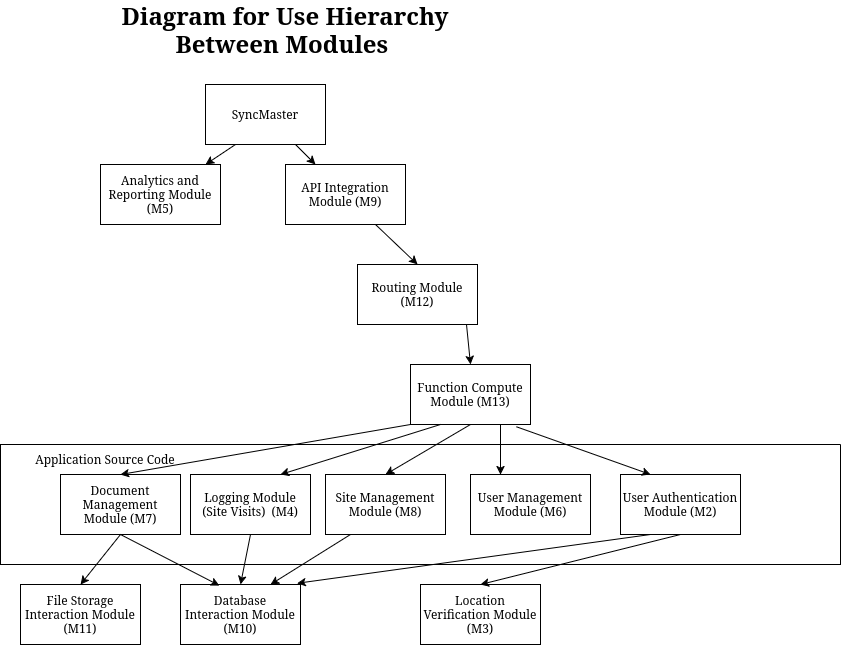
\includegraphics[width=0.7\textwidth]{userHierarchy.png}
  \caption{Use hierarchy among modules}
  \label{FigUH}
\end{figure}

%\section*{References}

\section{User Interfaces}

\wss{Design of user interface for software and hardware.  Attach an appendix if
needed. Drawings, Sketches, Figma}

\section{Design of Communication Protocols}

N/A

\section{Timeline}
Below is an timeline for the implementation of modules in this
project. The foundational modules User Authentication, User
Management, Database Interaction, Logging, Routing, and API
Integration will be developed first, as they form the core
infrastructure on which the remaining modules will depend. Once these
core modules are in place the other modules will be implemented. Task
responsibilities and deadlines are tracked on GitHub using GitHub
Issues \href{https://github.com/Spitgranger/SyncMaster/issues}{here}.
\begin{table}[H]
  \centering
  \begin{tabular}{|l|l|l|}
    \hline
    \textbf{Module} & \textbf{Responsible} & \textbf{Deadline} \\
    \hline
    M1: Audit and Compliance Module  & Akshit Gulia & January 31st, 2025 \\
    \hline
    M2: User Authentication Module    & Rafeed Iqbal & January 24th, 2025 \\
    \hline
    M3: Location Verification Module  & Rafeed Iqbal & January 31st, 2025 \\
    \hline
    M4: Logging Module                & Kyle D'Souza & January 24th, 2025 \\
    \hline
    M5: Analytics and Reporting Module & Akshit Gulia & January 31st, 2025 \\
    \hline
    M6: User Management Module        & Rafeed Iqbal & January 24th, 2025 \\
    \hline
    M7: Document Management Module    & Richard Fan & January 31st, 2025 \\
    \hline
    M8: Job Management Module         & Mitchell Hynes & January 31st, 2025 \\
    \hline
    M9: API Integration Module        & Richard Fan & January 24th, 2025 \\
    \hline
    M10: Database Interaction Module  & Kyle D'Souza & January 24th, 2025 \\
    \hline
    M11: Blob Storage Interaction Module & Kyle D'Souza & January 31st, 2025 \\
    \hline
    M12: Routing Module               & Kyle D'Souza & January 24th, 2025 \\
    \hline
    M13: Function Compute Module      & Kyle D'Souza & January 31st, 2025 \\
    \hline
  \end{tabular}
  \caption{Schedule for module implementation}
  \label{TblTimeline}
\end{table}

\bibliographystyle {plainnat}
\bibliography{../../../refs/References}

\newpage{}

\end{document}
